In this chapter you will learn how to make
free-standing wheat sourdough bread.

\begin{figure}[!htb]
  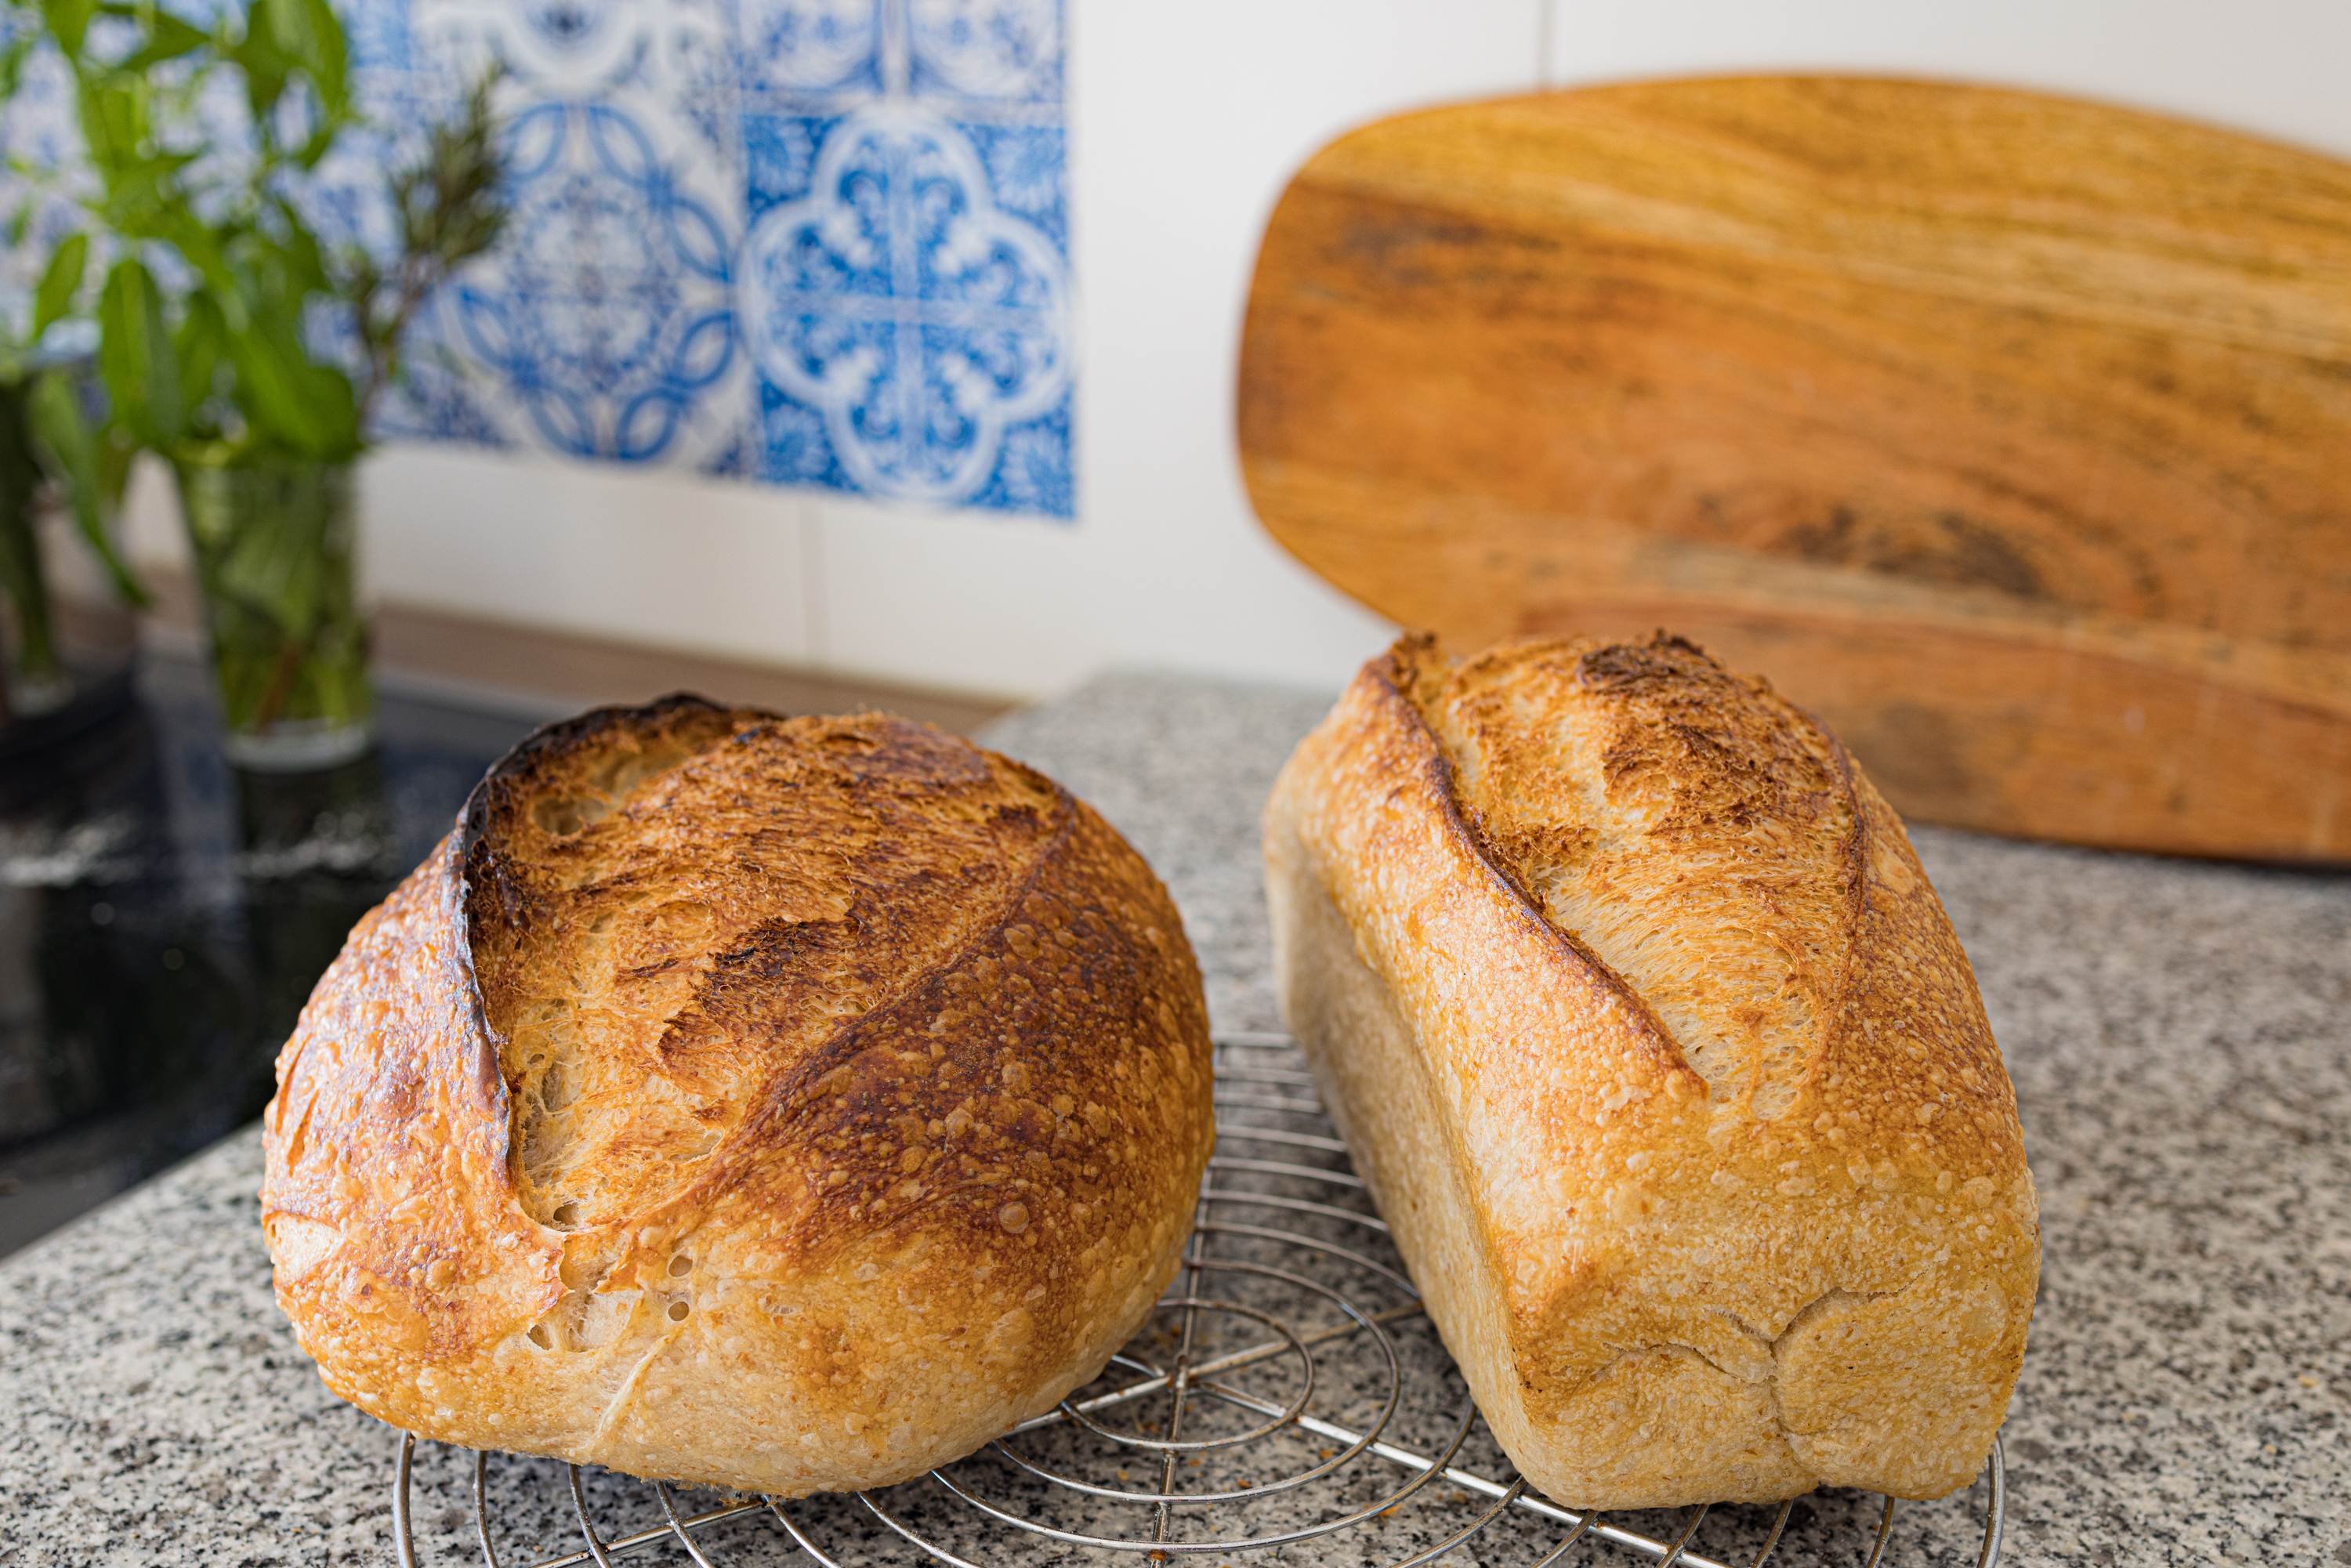
\includegraphics[width=\textwidth]{loaf-pan-free-standing.jpg}
  \caption{A free standing sourdough bread made with wheat flour}
\end{figure}

A free standing sourdough bread is my personal favorite
type of bread. It combines a great crunchy crust, superb
flavor and a soft fluffy crumb. This is the type of bread
that is being inhaled by my friends and family. Unfortunately
making this type of bread requires a lot more effort, patience
and technique than other types of bread. You have to perfectly
balance the fermentation process. You can not ferment for too
short and also not for too long. The techniques you need to
learn require a bit more skill. It took me several attempts
to get this right. One of the challenges I faced was that
I had the wrong flour. I didn't properly know how to use my oven.
When should I stop the fermentation? There is a lot of information
out there. I dug through most of it and have tried almost everything.
In many cases the information was wrong, in other cases I
found another valuable puzzle piece. Aggregating all this
information was one of my main motivations to start the bread code.
My key learning was that there there is no recipe that
you can blindly follow. You will always have to adapt the recipe
to your local available tools and environment.

But do not worry. After reading this chapter you will know
all the signs to look out for. You will be able to read your dough.
You will turn into a confident hobby baker that can bake bread
at home, high altitude, low altitude, in summer, in winter,
at your friend's place and even on vacation. Furthermore
you will know how to scale your production from 1 bread to 100 breads. If you
ever wanted to open up a bakery, consider this knowledge to
be your foundation.

Mastering this process will enable you to bake amazing bread without
ever buying yeast again.

\section{The process}

\begin{figure}[!htb]
  \includegraphics[width=\textwidth]{sourdough-process-overview.jpg}
  \caption{An overview of the whole sourdough process from start to finish}
\end{figure}

The whole process of making great sourdough bread starts with
readying your sourdough starter. The key to mastering
this process is to manage the fermentation process properly.
For this the basis is to have an active and healthy
sourdough starter.

Once your starter is ready you proceed to mix all the ingredients.
You want to homogenize your sourdough starter properly. This
way you ensure an even fermentation across your whole dough.

After a short break you will proceed and create dough strength.
Kneading will create a strong gluten network. This is essential
to properly trap the CO2 created during the fermentation.

Once you kneaded the bulk fermentation starts. Bulk fermentation
because you typically ferment multiple doughs together in one bulk.
Understanding when to stop this step will take some practice.
But nothing to worry, you will learn the exact signs to look out for.

Once this is completed you need to divide your large blob of
dough into smaller pieces and preshape each piece. This allows
you to apply more dough strength and shape more uniform loaves.

The proofing stage follows where you finish the fermentation process.
Depending on your time you can proof at room temperature or in the fridge.
Mastering proofing will turn your good loaf into a great loaf.

Lastly you will finish the whole process by baking. You will learn different
options on how to properly steam your dough. This way your
dough will have beautiful oven spring. During the second
stage of the bake you will finish building your crust.

All the steps rely on each other. You will need to get each of
the steps right to make the perfect bread.

\section{Readying your starter}
\section{Ingredients}
\section{Hydration}
\section{Autolyse}
\section{Fermentolyse}
\section{Dough strength}
\section{Controlling fermentation}
\section{Optional Preshaping}
\section{Shaping}
\section{Proofing}
\section{Scoring}
